\chapter{浮空器数学模型与故障分析}\label{chap:preliminary}
在推导浮空器的容错控制算法时,遇到的首要问题就是如何将浮空器的各项故障表达成数学形式并体现在模型中。本章中给出了本文所使用的浮空器数学模型,和浮空器平时可能遇到的一些常见故障及其数学表达。
\section{浮空器数学模型}
本文所研究的浮空器为外观型如图\newref{fig:airshipoverview}所示的螺旋桨矢量推进的浮空器。其横截面是四段欧拉螺线(Euler Spiral,又称羊角螺线)的一部分围成的闭合图形(图),这样能够保证体积一定的情况下所用布料最少。四个矢量推进螺旋桨均匀分布在最大半径纬度的周围。
\begin{figure}
    \centering
    
\includegraphics[width=0.5\textwidth]{figure/placeholder.png}
    \bicaption[fig:blimpcut]{欧拉螺线及浮空器横截面}{欧拉螺线及浮空器横截面}{Fig.}{Euler Spiral and Airship Cross-section}
\end{figure}

其机体坐标系、地面坐标系的建立过程和特性和模型已经在文献\citen{Chen20131748,zhanghao2014}中做了详细分析。相关参数也已经在本文前的符号列表中给出,这里仅简单将数学模型简单列举。
\begin{figure}
    \centering
    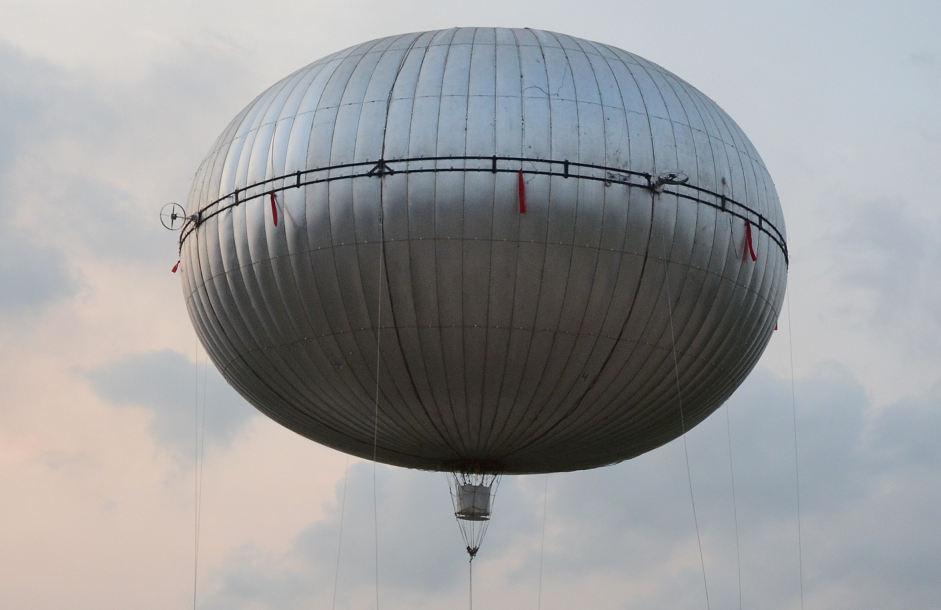
\includegraphics[width=0.7\textwidth]{airship.png}
    \bicaption[fig:airshipoverview]{螺旋桨矢量推进浮空器外观}{螺旋桨矢量推进浮空器外观}{Fig.}{The Apperance of Airship}
\end{figure}

令$x$, $y$, $z$分别为浮空器在地面坐标系下在$x$, $y$, $z$方向的位移,$\mathbf{x_1}=[x,y,z,\phi,\theta,\psi]^T$, $\mathbf{x_2}=[u,v,w,p,q,r]^T$,那么浮空器模型的状态空间形式为
\begin{equation}\label{eq:model1}
    \begin{cases}
    \dot{\mathbf{x}}_1 &= \mathbf{J}\dot{\mathbf{x}}_2 \\
    \mathbf{M}\dot{\mathbf{x}}_2 &= \mathbf{F_{gb}} + \mathbf{F_a} + \mathbf{F_i} + \mathbf{F_t}
    \end{cases}
\end{equation}
其中$\mathbf{J}$是坐标转换矩阵,其表达式为
\begin{equation}\label{eq:J}
\mathbf{J} = \left[\begin{matrix}
\mathbf{J_1}&\mathbf{O_{3\times3}}  \\
\mathbf{O_{3\times3}}&\mathbf{J_2} 
\end{matrix}\right]
\end{equation}

\begin{equation}\label{eq:J1}
\mathbf{J_1}=\left[
\begin{matrix}
\cos\psi\cos\theta&\cos\psi\sin\theta\sin\phi-\sin\psi\cos\phi&\cos\psi\sin\theta\cos\phi+\sin\psi\sin\phi\\
\sin\psi\cos\theta&\sin\psi\sin\theta\sin\phi+\cos\psi\cos\phi &\sin\psi\sin\theta\cos\phi-\cos\psi\sin\phi \\
-\sin\theta &\cos\theta\sin\phi&\cos\theta\cos\phi
\end{matrix}
\right]
\end{equation}

\begin{equation}\label{eq:J2}
\mathbf{J_2}=\left[
\begin{matrix}
1&\sin\phi\tan\theta&\cos\phi\tan\theta  \\
0&\cos\phi&-\sin\phi  \\
0&\sin\phi\sec\theta&\cos\phi\sec\theta  \\
\end{matrix}
\right]
\end{equation}

$\mathbf{M}$是惯性矩阵,其表达式为:
\begin{equation}\label{eq:M}
\mathbf{M}=\left[
\begin{matrix}
m+m_{11}&0&0&0&mz_G&-my_G  \\
0&m+m_{22}&0&0-mz_G&0&mx_G  \\
0&0&m+m_{33}&my_G&-mx_G&0  \\
0&-mz_G&my_G&I_x+m_{44}&0&0  \\
mz_G&0&-mx_G&0&I_y+m_{55}&0  \\
-my_G&mx_G&0&0&0&I_z+m_{66}  \\
\end{matrix}
\right]
\end{equation}

科氏力$\mathbf{F_i}$的表达式为
\begin{equation}\label{eq:Fi}
\mathbf{F_{i}}=\left[
\begin{matrix}
-(m+m_{33})wq+(m+m_{22})vr-mz_Gpr+mx_G(r^2+q^2)-my_Gpq  \\
-(m+m_{11})ur+(m+m_{33})wp-mz_Gqr+my_G(r^2+p^2)-mx_Gpq \\
-(m+m_{22})vp+(m+m_{11})uq-my_Gqr+mz_G(p^2+q^2)-mx_Gpr \\
(m_{55}-m_{66}-I_z+I_y)qr-my_G(pv-qu)+mz_G(ru-pw) \\
(m_{66}-m_{44}-I_x+I_z)pr-mz_G(qw-rv)+mx_G(pv-qu) \\
(m_{44}-m_{55}-I_y+I_z)qp-mx_G(ru-pw)+my_G(qw-rv)
\end{matrix}
\right]
\end{equation}

空气动力$\mathbf{F_a}$的表达式为
\begin{equation}\label{eq:Fa}
\mathbf{F_{a}}=\left[
\begin{matrix}
f_a\cdot\cos\Omega \\
f_a\cdot\sin\Omega \\
q_{\infty}\cdot C_z\cdot S_{ref} \\
-M_a\cdot\cos\Omega \\
M_a\cdot\sin\Omega \\
0\\
\end{matrix}
\right]
\end{equation}
其中
\begin{eqnarray}\label{eq:fa}
f_a &=& q_{\infty}\cdot C_x\cdot  S_{ref} \\
M_a &=& q_{\infty}\cdot C_{my}\cdot  S_{ref} \cdot L_{ref}
\end{eqnarray}

重力与浮力的合力$\mathbf{F_{gb}}$的表达式为
\begin{equation}\label{eq:Fgb}
\mathbf{F_{gb}}=\left[
\begin{matrix}
-(G-B)\mathrm{sin}\theta  \\
(G-B)\mathrm{sin}\phi\mathrm{cos}\theta \\
(G-B)\mathrm{cos}\phi\mathrm{cos}\theta \\
-(Gz_{G}-Bz_{B})\mathrm{sin}\phi\mathrm{cos}\theta \\
-(Gz_{G}-Bz_{B})\mathrm{sin}\theta-(Gx_{G}-Bx_{B})\mathrm{cos}\phi\mathrm{sin}\theta \\
(Gx_{G}-Bx_{B})\mathrm{sin}\phi\mathrm{cos}\theta
\end{matrix}
\right]
\end{equation}

浮空器的控制输入矢量$\mathbf{F_t}=[f_x, f_y, f_z, m_x, m_y, m_z]^T$的推导在文献\citen{zhanghao2014}中有详细提及。如果定义螺旋桨推力向上(即$z$轴负方向)的方向角为$0$,$\mu$为螺旋桨的方位角,其范围为$[-\pi,\pi]$,$f_i\text{ }(i=1,2,3,4)$为四个螺旋桨分别产生的推力大小。在矢量平面内,几个螺旋桨推进器的矢量推力可以分解为水平和垂直方向正交的两个力$f_{iH}$和$f_{iV}$,它们与矢量推力大小、矢量转角的关系为:
\begin{eqnarray}
f_{iH}&=&f_i\sin\mu_i \\
f_{iV}&=&-f_i\cos\mu_i
\end{eqnarray}
将$f_{iH}$和$f_{iV}$分解到坐标轴上,得到六维推力和推力力矩,如图\newref{fig:controlalloc}所示。
\begin{figure}
    \centering
    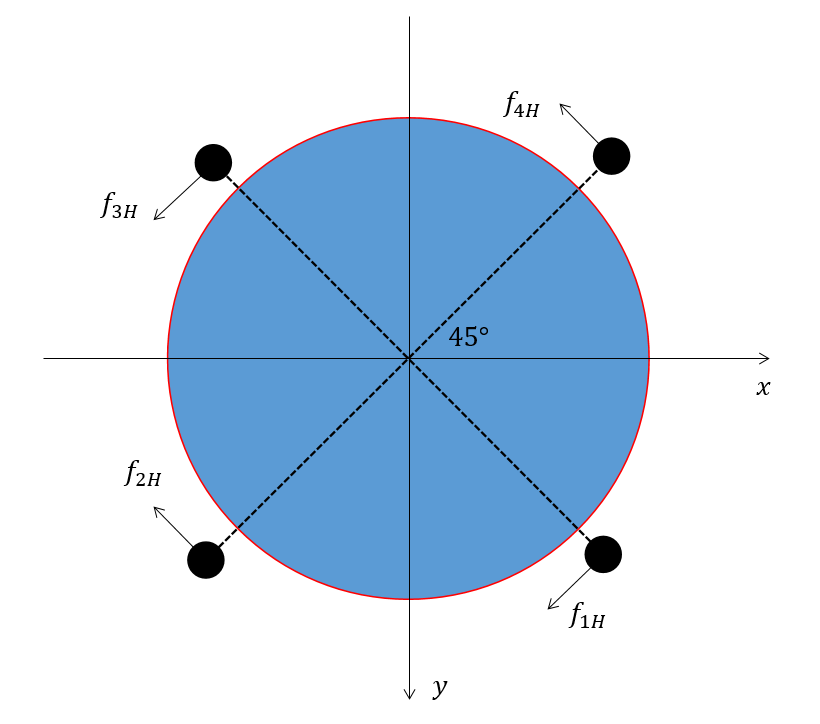
\includegraphics[width=0.7\textwidth]{figure/controlallocation.png}
    \bicaption[fig:controlalloc]{矢量推力局部坐标系和矢量角度定义}{矢量推力局部坐标系和矢量角度定义\cite{zhanghao2014}}{Fig.}{A sketch of the vectored thrusts}
\end{figure}
文献\citen{zhanghao2014}对$\mathbf{F_t}$和$f_{iH}$, $f_{iV}$, $\mu_i$之间的关系进行了详细的推导,这里仅给出结论如下:
\begin{equation}
    \mathbf{F_t}=\mathbf{D}F_{HV}
\end{equation}
其中
\begin{equation}\label{eq:D}
    \mathbf{D}=\left[\begin{matrix}
\rtwo&\rtwo&-\rtwo&-\rtwo&0&0&0&0\\
-\rtwo&\rtwo&\rtwo&-\rtwo&0&0&0&0\\
0&0&0&0&1&1&1&1\\
0&0&0&0&\rtwo R_p&\rtwo R_p&-\rtwo R_p&-\rtwo R_p\\
0&0&0&0&-\rtwo R_p&\rtwo R_p&\rtwo R_p&-\rtwo R_p\\
-R_p&-R_p&-R_p&-R_p&0&0&0&0\\
\end{matrix}
\right]
\end{equation}

\begin{equation}
    F_{HV} = \left[\begin{matrix}f_{1H}&f_{2H}&f_{3H}&f_{4H}&f_{1V}&f_{2V}&f_{3V}&f_{4V}\end{matrix}
\right]^T
\end{equation}

这里$\mathbf{D}$为控制分配矩阵,$F_{HV}$为中间控制量。

在实际进行控制时,控制器计算得出控制量$\mathbf{F_t}$后,通过$\mathbf{D}$的伪逆矩阵$\mathbf{D}^{\dagger}$和\neweqref{eq:fthv}可以计算得出每个螺旋桨实际需求的分力$F_{T_{HV}}$,再通过\neweqref{eq:fi}和\neweqref{eq:miui}计算出各个螺旋桨的实际输出量,求得每个螺旋桨实际所需的推力和转角大小。
\begin{equation}\label{eq:fthv}
    F_{T_{HV}} = \mathbf{D}^{\dagger}\mathbf{F_t}
\end{equation}

\begin{equation}\label{eq:fi}
    f_i = \sqrt{f_{iH}^2+f_{iV}^2}, \qquad (i=1,2,3,4)
\end{equation}

\begin{equation}\label{eq:miui}
    \mu_i = \tan^{-1}\left(\frac{f_{iH}}{f_{iV}}\right), \qquad (i=1,2,3,4)
\end{equation}

\section{浮空器故障的数学形式分析}
\subsection{附加质量问题}
不同于高速飞行器,浮空器的附加质量非常明显。事实上,任何在流体中运动的物体都会对流体产生作用力,这个作用力会对物体本身产生反作用力,造成物体的动量变化\cite{mueller2004development}。为了仍使物体维持原定速度运行,人们引入了附加质量来抵消这部分流体反作用力。在传统的飞机模型中,因为飞机本身质量很大,这部分空气反作用力是可以被忽略的。然而对于浮空器来说,这部分反作用力和其质量几乎同属一个数量级,因此不能被忽略。

附加质量的数学形式就体现在惯性矩阵$\mathbf{M}$中。如果没有附加质量,那么浮空器的惯性矩阵应为对角阵:
\begin{equation}
    \left[\begin{matrix}
    m&&&&&\\
    &m&&&&\\
    &&m&&&\\
    &&&I_x&&\\
    &&&&I_y&\\
    &&&&&I_z\\
    \end{matrix}\right]
\end{equation}

引入附加质量后,需要注意的是每个飞行器的惯性矩阵都因其形状而各自不同,式\neweqref{eq:M}所示的附加质量矩阵只适用于本文的或与本文中研究对象形状相似的物体。

\subsection{气动参数不确定问题}
气动参数不确定也是浮空器研究中经常面临的一类问题。这里的气动参数主要指式\neweqref{eq:Fa}-\neweqref{eq:fa}中的参数$C_x$, $C_z$和$C_{my}$。这几个参数与浮空器当前的气动迎角$\Omega$有关,通常测量方法是在风洞中每隔一段角度测出对应迎角的气动系数,得到一个参数表。对于某一未测量角度的气动参数,则是根据已知的参数表进行线性插值求得。这样获取的气动参数的不准确性在于

\begin{itemize}
    \item 由于风速不确定的原因,实际的迎角不易准确测得。
    \item 即使迎角可以准确测到,由于浮空器的形变等原因,其气动系数相对于风洞中的测量值可能会有变化。
    \item 由于在风洞中不可能对每个角度都进行测量,因此在对气动系数进行线性插值时会产生误差。
\end{itemize}

以上原因造成了实际中使用的$C_x$,$C_z$与$C_{my}$都会与真实值有出入,因此气动参数不确定也是浮空器研究面临的一个难点。在本文的后续仿真中,我们以增加一个正态分布扰动来表示真实的气动系数。

\subsection{外部扰动问题}
外部扰动指的是除了已知的控制输入外,空气额外作用在浮空器上的力。对于浮空器来说,通常最大的外部扰动来源是风的影响,同时也可能有一些湍流等作用。外部扰动分为匹配(matched)扰动和不匹配(unmatched)扰动。匹配扰动表示可以将这部分扰动归并到执行机构扰动中考虑,并在执行机构中做相应的补偿就可以了;而不匹配扰动则无法通过执行机构做直接补偿。浮空器的外部扰动的数学模型是在模型\neweqref{eq:model1}中的动力学方程中直接添加,即

\begin{equation}
    \mathbf{M}\dot{\mathbf{x}}_2 = \mathbf{F_{gb}} + \mathbf{F_a} + \mathbf{F_i} + \mathbf{F_t} + \mathbf{d}
\end{equation}

其中$\mathbf{d}$为外部扰动。

\subsection{执行机构故障}
执行机构故障也是一种常见的系统错误。由于平流层浮空器通常工作在十分恶劣的环境下,因此任何执行机构,包括螺旋桨和舵面,都很容易失效。由于本文的研究对象的执行机构是螺旋桨,所以本文仅给出了针对螺旋桨一些常见故障的数学建模。

螺旋桨遇到的问题可以归结为效率损失、输出偏移,卡顿和失效等几类。假设某个执行机构$i$的期望输出为$\upsilon_i$, 其输出效率为$\varepsilon_i$,输出偏移为$\bar{\upsilon_i}$,那么有
\begin{equation}\label{eq:outputeff}
    u_{ai} = \varepsilon_i(t)\upsilon_i+\bar{\upsilon_i}
\end{equation}

对于上述提到的各种故障,可总结其数学模型于表\newref{tab:faultmodel}。
\begin{table}[ht]
    \centering
	\bicaption[tab:faultmodel]{螺旋桨故障及其数学模型}{螺旋桨故障及其数学模型}{Table}{Thrust fault classifications and math models}
	\vspace{0.5em}
	\begin{tabular}{lll}
		\toprule
		故障类型&$\varepsilon_i(t)$&$\bar{\upsilon}_i$ \\
		\midrule
		正常&$\varepsilon_i(t)=1$&$\bar{\upsilon}_i=0$\\
		效率损失&$\varepsilon_i(t)<1$&$\bar{\upsilon}_i=0$\\
		输出偏移&$\varepsilon_i(t)=1$&$\bar{\upsilon}_i\neq0$\\
		卡顿&$\varepsilon_i(t)=0$&$\upsilon_i\neq0$\\
		失效&$\varepsilon_i(t)=0$&$\upsilon_i=0$\\
		\bottomrule
	\end{tabular}
\end{table}

浮空器的实际输出$\mathbf{F_t}$可用式\neweqref{eq:inputtrans}表示

\begin{equation}\label{eq:inputtrans}
    \mathbf{F_t} = \mathbf{Du_a} = \mathbf{D}[EF_{HV} + \bar{\upsilon}]
\end{equation}

其中

\begin{equation*}
    E = \left[\begin{matrix}
    \varepsilon_1&&&&&&&\\
    &\varepsilon_2&&&&&&\\
    &&\varepsilon_3&&&&&\\
    &&&\varepsilon_4&&&&\\
    &&&&\varepsilon_5&&&\\
    &&&&&\varepsilon_6&&\\
    &&&&&&\varepsilon_7&\\
    &&&&&&&\varepsilon_8\\
    \end{matrix}\right]
\end{equation*}

\begin{equation*}
    \bar{\upsilon} = \left[\begin{matrix}
    \bar{\upsilon}_1&\bar{\upsilon}_2&\cdots&\bar{\upsilon}_8
    \end{matrix}\right]^T
\end{equation*}


\section{本章小结}
本章简要介绍了本文的研究对象浮空器的形状。同时引入了浮空器数学模型和它不同于飞机的独特之处。在第二节中介绍了浮空器运行时可能遇到的各类故障和扰动、以及它们在浮空器模型方程中的数学体现,为后文设计浮空器的容错控制算法做了坚实的铺垫,打下了良好的基础。